\chapter{STP}
\section{Issues with redundancy}
Multiple cabled paths between switches provide physical redundancy in a switched network. This improves the reliability and availability of the network. However, when there is no spanning tree implementation on the switches, a Layer 2 loop occurs. A Layer 2 loop can result in the three primary issues:
\begin{itemize}
\item Duplicate unicast frames
\item MAC database instability
\item Broadcast storm
\end{itemize}
\subsection{Multiple-frame transmission}
Broadcast frames are not the only type of frames that are affected by loops. Unknown unicast frames sent onto a looped network can result in duplicate frames arriving at the destination device. An unknown unicast frame is when the switch does not have the destination MAC address in its MAC address table and must forward the frame out all ports, except the ingress port.
\subsection{MAC Database Instability}
Ethernet frames do not have a time to live (TTL) attribute. As a result, if there is no mechanism enabled to block continued propagation of these frames on a switched network, they continue to propagate between switches endlessly. \par 
Broadcast frames are forwarded out all switch ports, except the original ingress port. If there is more than one path to the destination, the frames may be forwarded back to the original switch, and create an endless loop. When a loop occurs, the MAC address table on a switch to constantly change with the updates from the broadcast frames, which results in MAC database instability. \par 
See this \href{https://ccnav6.com/s3/course/module2/2.1.1.2/2.1.1.2.html}{link} for more explanation.
\subsection{Broadcast storm}
A broadcast storm occurs when there are so many broadcast frames caught in a Layer 2 loop that all available bandwidth is consumed. Consequently, no bandwidth is available for legitimate traffic and the network becomes unavailable for data communication. This is an effective denial of service (DoS).\par 
There are other consequences of broadcast storms. Because broadcast traffic is forwarded out every port on a switch, all connected devices have to process all the broadcast traffic that is being flooded endlessly around the looped network. This can cause the end device to malfunction because of the processing requirements needed to sustain such a high traffic load on the NIC.
\section{Operation}
\subsection{Port Roles}
IEEE 802.1D STP and RSTP use the Spanning Tree Algorithm (STA) to determine which switch ports on a network must be put in blocking state to prevent loops from occurring. The STA designates a single switch as the root bridge and uses it as the reference point for all path calculations (see figure \ref{STP-operation}). \par 
\begin{figure}[hbtp]
\centering
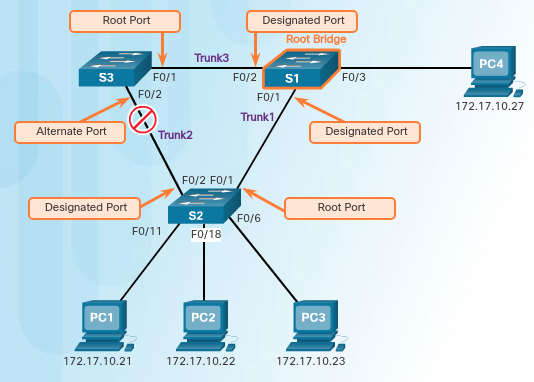
\includegraphics[width=0.8\textwidth]{pictures/STP-operation.png}
\caption{The STA designates a single switch as the root bridge and uses it as the reference point for all path calculations.}
\label{STP-operation}
\end{figure}
After  the root bridge has been determined, the STA calculates the shortest path to the root bridge, while each switch uses the STA to determine which ports to block.  When the STA has determined which paths are most desirable relative to each switch, it assigns port roles to the participating switch ports:
\begin{itemize}
\item \textbf{Root port} -- Switch ports closest to the root bridge in terms of overall cost to the root bridge.
\item \textbf{Designated port} -- All non-root ports that are still permitted to forward traffic on the network.
\item \textbf{Alternate port} -- Alternate ports and backup ports are in discarding or blocking state to prevent loops. 
\end{itemize}
Sometimes, the administrator wants to determine port roles without calculating port cost. He/She should keep in mind the following tips:
\begin{itemize}
\item There can only be one root port per non-root switch
\item If one end of a segment (the link between two switches) is a root port, then the other end is a designated port.
\item All ports on the root bridge are designated ports.
\item Alternate ports are selected only on segments where neither end is a root port.
\end{itemize}
\subsection{Root bridge}
Every switch has its own BID and a root ID:
\subsection{Bridge ID (BID)}
This field is used to uniquely identify the switch in the election process. It includes the priority, extended system ID, and MAC address (see figure \ref{BID}). The bridge priority value is automatically assigned, but can be modified by the administrator. The extended system ID is used to specify a VLAN ID or a multiple spanning tree protocol (MSTP) instance ID. 
\begin{figure}[hbtp]
\centering
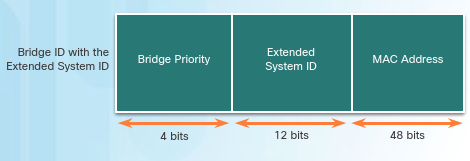
\includegraphics[width=0.6\textwidth]{pictures/BID.png}
\caption{BID fields}
\label{BID}
\end{figure}
The bridge priority is a customizable value that can be used to influence which switch becomes the root bridge. The switch with the lowest priority, which implies the lowest BID, becomes the root bridge because a lower priority value takes precedence. The default priority value for all Cisco switches is the decimal value 32768. The range is 0 to 61440 in increments of 4096.\par 
The extended system ID reserves the rightmost 12 bits for the VLAN ID and the far left 4 bits for the bridge priority. This explains why the bridge priority value can only be configured in multiples of 4096, or $2^12$.\par 
When two switches are configured with the same priority and have the same extended system ID, the switch having the MAC address with the lowest value, expressed in hexadecimal, will have the lower BID. Initially, all switches are configured with the same default priority value. The MAC address is then the deciding factor as to which switch is going to become the root bridge. 
\subsubsection{root ID}
This field indicates the BID of the root bridge. When a switch first boots, the root ID is the same as the bridge ID (BID). However, as the election occurs, the lowest BID replaces the local root ID to identify the root bridge.
\subsubsection{Election process}
All switches in the broadcast domain participate in the election process. After a switch boots, it begins to send out BPDU frames every two seconds. These BPDUs contain the switch BID and the root ID.\par 
Assuming that switch A,B,C,D resides in the same STP domain. As the switch A forward its BPDU frames, adjacent switch B reads the root ID information from the BPDU frames. If the root ID from the BPDU received is lower than the root ID on B, then the B updates its root ID, identifying the A as the root bridge. Switch B then forwards new BPDU frames with the lower root ID to switch C.\par 
The same process repeats, switch C compares its current root ID with the root ID identified in the frames, and then updates its current root ID if needed. Eventually, the switch with the lowest BID ends up being identified as the root bridge for the spanning tree instance.
\subsection{Port role decision}
After the root bridge is elected, the STA determines port roles on interconnecting links.\par 
The root bridge automatically configures all of its switch ports in the designated role. Non-root switches transition ports with the lowest root path cost to root ports, and the other to either  designated or alternate port (because there can only be one root port per non-root switch). \par 
Next step is to decide which port to configure as a designated or alternative port. On the segment, where root ports have already been defined, two switches exchange BPDU frames, which contain the BID. Generally, the switch with the lower BID has its port configured as a designated port while the other has its port configured as an alternate port. However, keep in mind that the first priority is the lowest path cost to the root bridge and that the sender’s BID is used only if the port costs are equal.
\subsection{Root path cost}
The STA considers both path and port costs when determining which ports to block.The path information, known as the internal root path cost, is determined by summing up the individual port costs along the path from the switch to the root bridge. The default port costs are defined by the speed at which the port operates. 10 Gb/s Ethernet ports have a port cost of 2, 1 Gb/s Ethernet ports have a port cost of 4, 100 Mb/s Fast Ethernet ports have a port cost of 19, and 10 Mb/s Ethernet ports have a port cost of 100.\par 
Switches send BPDUs, which include the root path cost. This is the cost of the path from the sending switch to the root bridge. When a switch receives the BPDU, it adds the ingress port cost of the segment to determine its internal root path cost.
\subsection{BPDU frame}
A Bridge Protocol Data Units (BPDU) is a frame exchanged by switches for STP. The spanning tree algorithm depends on the exchange of BPDUs to determine a root bridge. BPDUs have a destination MAC address of 01:80:C2:00:00:00, which is a multicast address for the spanning tree group.  A BPDU frame contains 12 distinct fields:
\begin{itemize}
\item The first four fields identify the protocol, version, message type, and status flags.
\item The next four fields are \textit{root ID}, \textit{bridge ID (BID)}, root path cost. They are  used to identify the root bridge and the root path cost to the root bridge.
\item The last four fields are all timer fields that determine how frequently BPDU messages are sent and how long the information received through the BPDU process is retained.
\end{itemize}
\section{Types of STP}
\begin{itemize}
\item \textbf{STP} -- This is the original IEEE 802.1D version. The protocol assumes one spanning tree instance for the entire bridged network.
\item \textbf{PVST+} -- This is a Cisco enhancement of STP that provides a separate 802.1D spanning tree instance for each VLAN configured in the network.
\item \textbf{802.1D-2004} -- This is an updated version of the STP standard, incorporating IEEE 802.1w.
\item \textbf{RSTP or IEEE 802.1w} -- This is an evolution of STP.
\item \textbf{Rapid PVST+} -- This is a Cisco enhancement of RSTP that uses PVST+.
\item \textbf{MSTP} -- Multiple Spanning Tree Protocol. This is an IEEE standard inspired by the earlier Cisco proprietary Multiple Instance STP (MISTP) implementation. MSTP maps multiple VLANs into the same spanning tree instance. The Cisco implementation of MSTP is MST, which provides up to 16 instances of RSTP
\end{itemize}
\subsection{Port states and PVST+ Operation}
To facilitate the learning of the logical spanning tree, each switch port transitions through five possible port states and three BPDU timers:
\begin{table}[h!]
\centering
\caption{Five port states in PVST+}
\label{PVST-port-state}
\begin{tabular}{|p{0.25\textwidth}|l|l|l|l|l|}
\hline
                                                    & \multicolumn{5}{c|}{Port states}                        \\ \hline
Operation allowed                                   & Blocking & Listening & Learning & Forwarding & Disabled \\ \hline
Learn MAC addresses                                 & YES      & YES       & YES      & YES        & NO       \\ \hline
Forward data frames received on interface           & NO       & NO        & YES      & YES        & NO       \\ \hline
Forward data frames switched from another interface & NO       & NO        & NO       & YES        & NO       \\ \hline
Receive and process BPDUs                           & NO       & NO        & NO       & YES        & NO       \\ \hline
\end{tabular}
\end{table}
\subsection{Rapid PVST+}
Rapid PVST+ is the Cisco implementation of RSTP on a per-VLAN basis. An independent instance of RSTP runs for each VLAN.\par 
RSTP does not have a blocking port state. Port states are defined as discarding, learning, or forwarding. RSTP also speeds the recalculation of the spanning tree when the Layer 2 network topology changes. If a port is configured to be an alternate port or a backup port, it can immediately change to a forwarding state without waiting for the network to converge.\par 
RSTP introduces new types of port: edge port. An RSTP edge port is a switch port that is never intended to be connected to another switch. It immediately transitions to the forwarding state when enabled. The RSTP edge port concept corresponds to the PVST+ PortFast feature. An edge port is directly connected to an end station and assumes that no switch device is connected to it.